\subsubsection{Suporte superior}
El soporte superior (fig. \ref{fig:Superior_orginal}) es el que recibe la mayor carga en la estructura, ya que debe soportar el peso de la estructura vertical (soportes, brazo robótico, varillas). Para ello se debe realizar un análisis de carga y deformación previos para verificar si la forma del soporte es la adecuada para tolerar los esfuerzos.
\begin{figure}[H]
    \centering
    \begin{subfigure}[b]{0.45\textwidth}
        \centering
        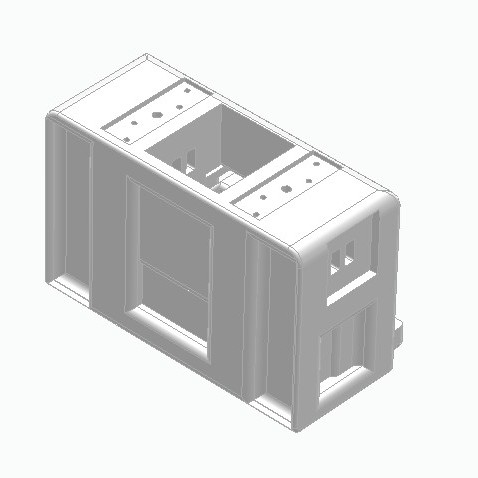
\includegraphics[width=\textwidth]{img/Superior_frente.jpg}
        \caption{Frente del soporte superior.}
        \label{fig:izaje_desacoplado}
    \end{subfigure}
    \hspace{0.02\textwidth}
    \begin{subfigure}[b]{0.45\textwidth}
        \centering
        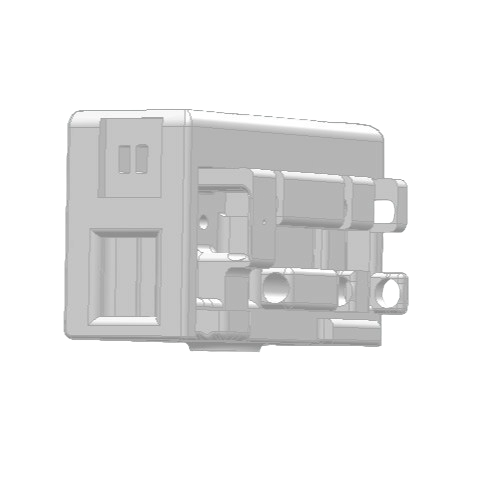
\includegraphics[width=\textwidth]{img/superior_atras.jpg}
        \caption{Posterior del soporte superior.}
        \label{fig:izaje_acoplado}
    \end{subfigure}
     \caption{Soporte superior.}
    \label{fig:Superior_orginal}
\end{figure}
Para realizar el análisis de esfuerzos y deformación se simplificó la pieza ya que el solver del software utilizado no podía procesar y analizar geometrías tan complejas como la planteada. Además se tomaron las propiedades del filamento plástico PETG de impresión 3D para hacer un correcto análisis.\\
En la siguiente figura se pueden observar las fuerzas aplicadas, las mismas contemplan una carga máxima de 3.5kg. Las fuerzas son aplicadas en las secciones indicadas en la imagen y divididas en dos para la parte superior y en tres para la parte inferior.\\
\begin{figure}[H]
    \centering
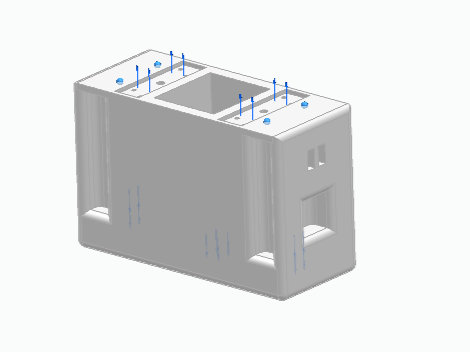
\includegraphics[width=0.65\textwidth]{img/Fuerzas_superiores.png} \par
    \caption{\textit{Fuerzas aplicadas para el análisis}}
    \label{fig:fuerzas_sup}
\end{figure}
A continuación se muestran los resultados obtenidos. \\
\begin{figure}[H]
    \centering
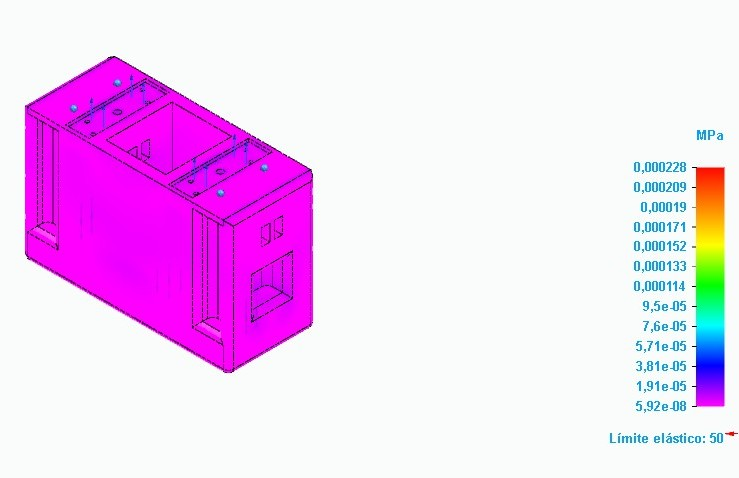
\includegraphics[width=0.65\textwidth]{img/completo_sin_mallar.jpg} \par
    \caption{\textit{Análisis de tensión de Von Misses.}}
    \label{fig:sup_analisis_tension}
\end{figure} 
\begin{figure}[H]
    \centering
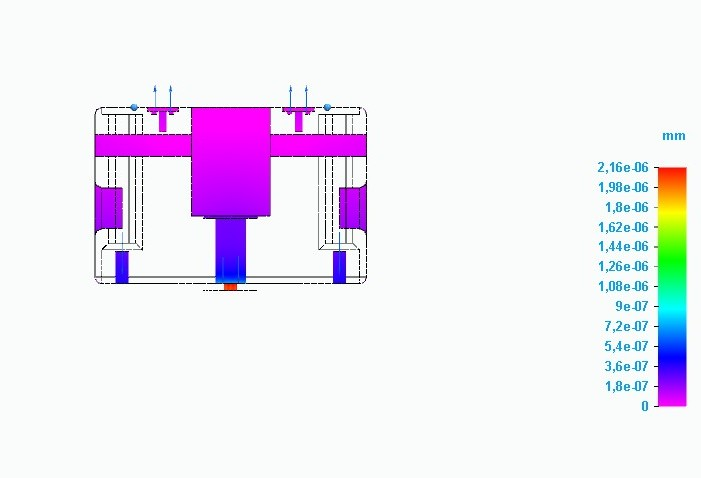
\includegraphics[width=0.65\textwidth]{img/Corte_transv_sin_mallado_def.jpg} \par
    \caption{\textit{Análisis de deformación.}}
    \label{fig:sup_analisis_def}
\end{figure}
Como se puede observar en las imágenes, la tensión está muy por debajo de la tensión de rotura y las deformaciones son prácticamente insignificantes, por lo que se puede concluir que el diseño es aplicable.\\


\subsubsection{Suporte medio}
Este soporte se desplaza por el movimiento de la varilla, además es en donde se encuentra el brazo robótico y la cámara. Cuenta con canales internos para el montaje de los cables. \\
\begin{figure}[H]
    \centering
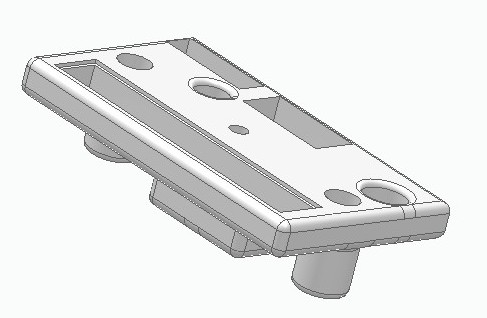
\includegraphics[width=0.65\textwidth]{img/medio.jpg} \par
    \caption{\textit{Soporte medio.}}
    \label{fig:soporte_medio}
\end{figure}


\subsubsection{Suporte inferior}
Este soporte cierra la estructura vertical, en el van los extremos de las varillas trefiladas y la varilla roscada y el final de carrera correspondiente. También cuenta con canales internos para el montaje de los cables. \\
\begin{figure}[H]
    \centering
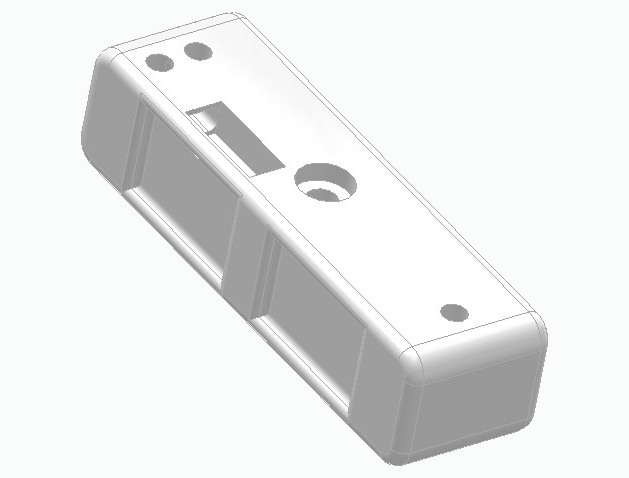
\includegraphics[width=0.65\textwidth]{img/inferior_completo.jpg} \par
    \caption{\textit{Soporte inferior.}}
    \label{fig:soporte_inferior}
\end{figure}

\subsubsection{Brazo robótico}
Para el diseño del brazo robótico se tienen 2 partes principales, el cuerpo del brazo y el efector final o gripper. \\
\begin{figure}[H]
    \centering
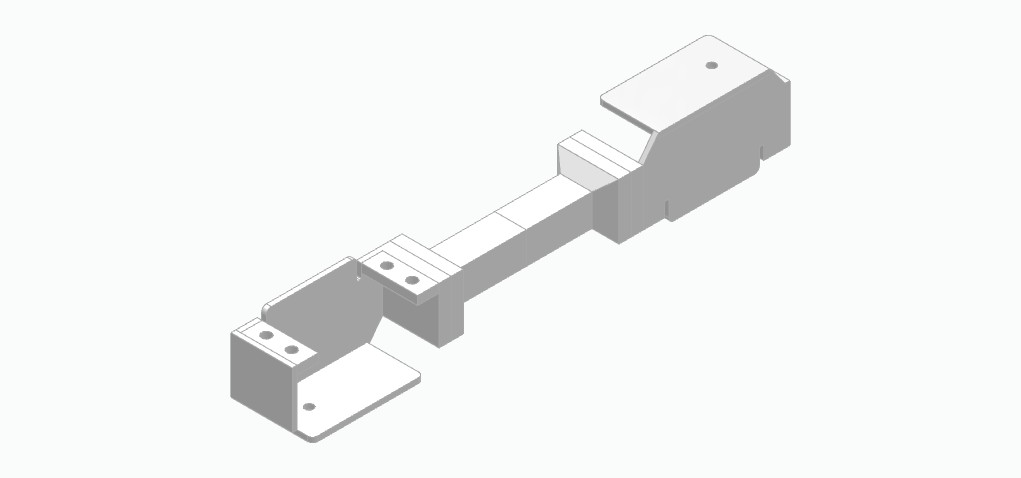
\includegraphics[width=0.65\textwidth]{img/brazo_medio.jpg} \par
    \caption{\textit{Cuerpo del brazo.}}
    \label{fig:brazo}
\end{figure}
El diseño del gripper tiene en cuenta un sistema de transmisión piñon-cremallera para el agarre. 
\begin{figure}[H]
    \centering
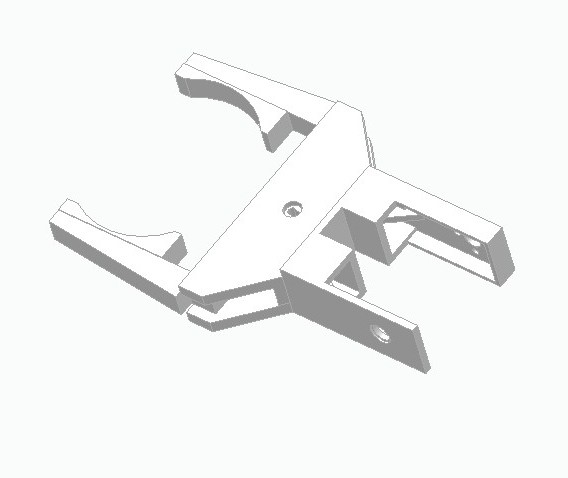
\includegraphics[width=0.65\textwidth]{img/pinza.jpg} \par
    \caption{\textit{Gripper.}}
    \label{fig:gripper}
\end{figure}


